% Options for packages loaded elsewhere
\PassOptionsToPackage{unicode}{hyperref}
\PassOptionsToPackage{hyphens}{url}
\PassOptionsToPackage{dvipsnames,svgnames,x11names}{xcolor}
%
\documentclass[
  12pt]{article}

\usepackage{amsmath,amssymb}
\usepackage{iftex}
\ifPDFTeX
  \usepackage[T1]{fontenc}
  \usepackage[utf8]{inputenc}
  \usepackage{textcomp} % provide euro and other symbols
\else % if luatex or xetex
  \usepackage{unicode-math}
  \defaultfontfeatures{Scale=MatchLowercase}
  \defaultfontfeatures[\rmfamily]{Ligatures=TeX,Scale=1}
\fi
\usepackage{lmodern}
\ifPDFTeX\else  
    % xetex/luatex font selection
\fi
% Use upquote if available, for straight quotes in verbatim environments
\IfFileExists{upquote.sty}{\usepackage{upquote}}{}
\IfFileExists{microtype.sty}{% use microtype if available
  \usepackage[]{microtype}
  \UseMicrotypeSet[protrusion]{basicmath} % disable protrusion for tt fonts
}{}
\makeatletter
\@ifundefined{KOMAClassName}{% if non-KOMA class
  \IfFileExists{parskip.sty}{%
    \usepackage{parskip}
  }{% else
    \setlength{\parindent}{0pt}
    \setlength{\parskip}{6pt plus 2pt minus 1pt}}
}{% if KOMA class
  \KOMAoptions{parskip=half}}
\makeatother
\usepackage{xcolor}
\setlength{\emergencystretch}{3em} % prevent overfull lines
\setcounter{secnumdepth}{5}
% Make \paragraph and \subparagraph free-standing
\ifx\paragraph\undefined\else
  \let\oldparagraph\paragraph
  \renewcommand{\paragraph}[1]{\oldparagraph{#1}\mbox{}}
\fi
\ifx\subparagraph\undefined\else
  \let\oldsubparagraph\subparagraph
  \renewcommand{\subparagraph}[1]{\oldsubparagraph{#1}\mbox{}}
\fi


\providecommand{\tightlist}{%
  \setlength{\itemsep}{0pt}\setlength{\parskip}{0pt}}\usepackage{longtable,booktabs,array}
\usepackage{calc} % for calculating minipage widths
% Correct order of tables after \paragraph or \subparagraph
\usepackage{etoolbox}
\makeatletter
\patchcmd\longtable{\par}{\if@noskipsec\mbox{}\fi\par}{}{}
\makeatother
% Allow footnotes in longtable head/foot
\IfFileExists{footnotehyper.sty}{\usepackage{footnotehyper}}{\usepackage{footnote}}
\makesavenoteenv{longtable}
\usepackage{graphicx}
\makeatletter
\def\maxwidth{\ifdim\Gin@nat@width>\linewidth\linewidth\else\Gin@nat@width\fi}
\def\maxheight{\ifdim\Gin@nat@height>\textheight\textheight\else\Gin@nat@height\fi}
\makeatother
% Scale images if necessary, so that they will not overflow the page
% margins by default, and it is still possible to overwrite the defaults
% using explicit options in \includegraphics[width, height, ...]{}
\setkeys{Gin}{width=\maxwidth,height=\maxheight,keepaspectratio}
% Set default figure placement to htbp
\makeatletter
\def\fps@figure{htbp}
\makeatother

\addtolength{\oddsidemargin}{-.5in}%
\addtolength{\evensidemargin}{-1in}%
\addtolength{\textwidth}{1in}%
\addtolength{\textheight}{1.7in}%
\addtolength{\topmargin}{-1in}%

\usepackage{booktabs}
\usepackage{longtable}
\usepackage{array}
\usepackage{multirow}
\usepackage{wrapfig}
\usepackage{float}
\usepackage{colortbl}
\usepackage{pdflscape}
\usepackage{tabu}
\usepackage{threeparttable}
\usepackage{threeparttablex}
\usepackage[normalem]{ulem}
\usepackage{makecell}
\usepackage{xcolor}
\makeatletter
\makeatother
\makeatletter
\makeatother
\makeatletter
\@ifpackageloaded{caption}{}{\usepackage{caption}}
\AtBeginDocument{%
\ifdefined\contentsname
  \renewcommand*\contentsname{Table of contents}
\else
  \newcommand\contentsname{Table of contents}
\fi
\ifdefined\listfigurename
  \renewcommand*\listfigurename{List of Figures}
\else
  \newcommand\listfigurename{List of Figures}
\fi
\ifdefined\listtablename
  \renewcommand*\listtablename{List of Tables}
\else
  \newcommand\listtablename{List of Tables}
\fi
\ifdefined\figurename
  \renewcommand*\figurename{Figure}
\else
  \newcommand\figurename{Figure}
\fi
\ifdefined\tablename
  \renewcommand*\tablename{Table}
\else
  \newcommand\tablename{Table}
\fi
}
\@ifpackageloaded{float}{}{\usepackage{float}}
\floatstyle{ruled}
\@ifundefined{c@chapter}{\newfloat{codelisting}{h}{lop}}{\newfloat{codelisting}{h}{lop}[chapter]}
\floatname{codelisting}{Listing}
\newcommand*\listoflistings{\listof{codelisting}{List of Listings}}
\makeatother
\makeatletter
\@ifpackageloaded{caption}{}{\usepackage{caption}}
\@ifpackageloaded{subcaption}{}{\usepackage{subcaption}}
\makeatother
\makeatletter
\@ifpackageloaded{tcolorbox}{}{\usepackage[skins,breakable]{tcolorbox}}
\makeatother
\makeatletter
\@ifundefined{shadecolor}{\definecolor{shadecolor}{rgb}{.97, .97, .97}}
\makeatother
\makeatletter
\makeatother
\makeatletter
\makeatother
\ifLuaTeX
  \usepackage{selnolig}  % disable illegal ligatures
\fi
\usepackage[]{natbib}
\bibliographystyle{agsm}
\IfFileExists{bookmark.sty}{\usepackage{bookmark}}{\usepackage{hyperref}}
\IfFileExists{xurl.sty}{\usepackage{xurl}}{} % add URL line breaks if available
\urlstyle{same} % disable monospaced font for URLs
\hypersetup{
  pdftitle={Looking at Non-Linear Dimension Reductions as Models in the Data Space},
  pdfauthor={Jayani P.G. Lakshika; Dianne Cook; Paul Harrison; Michael Lydeamore; Thiyanga S. Talagala},
  pdfkeywords={high-dimensional data, dimension
reduction, triangulation, hexagonal binning, low-dimensional
manifold, manifold learning, tour, data vizualization},
  colorlinks=true,
  linkcolor={blue},
  filecolor={Maroon},
  citecolor={Blue},
  urlcolor={Blue},
  pdfcreator={LaTeX via pandoc}}


\begin{document}


\def\spacingset#1{\renewcommand{\baselinestretch}%
{#1}\small\normalsize} \spacingset{1}

%%%%%%%%%%%%%%%%%%%%%%%%%%%%%%%%%%%%%%%%%%%%%%%%%%%%%%%%%%%%%%%%%%%%%%%%%%%%%%

\title{\bf Looking at Non-Linear Dimension Reductions as Models in the
Data Space}
\author{
Jayani P.G. Lakshika\\
Econometrics \& Business Statistics, Monash University\\
and\\Dianne Cook\\
Econometrics \& Business Statistics, Monash University\\
and\\Paul Harrison\\
MGBP, BDInstitute, Monash University\\
and\\Michael Lydeamore\\
Econometrics \& Business Statistics, Monash University\\
and\\Thiyanga S. Talagala\\
Statistics, University of Sri Jayewardenepura\\
}
\maketitle

\bigskip
\bigskip
\begin{abstract}
Nonlinear dimension reduction (NLDR) techniques such as tSNE, and UMAP
provide a low-dimensional representation of high-dimensional (high-D)
data using non-linear transformation. The methods and parameter choices
can create wildly different representations, making it difficult to
decide which is best, or whether any or all are accurate or misleading.
NLDR often exaggerates random patterns, sometimes due to the samples
observed. But NLDR views have an important role in data analysis
because, if done well, they provide a concise visual (and conceptual)
summary of high-D distributions. To help evaluate the NLDR we have
developed an algorithm to show the 2D NLDR model in the high-D space,
viewed with a tour. One can see if the model fits everywhere or better
in some subspaces, or completely mismatches the data. It is used to
evaluate which 2D layout is the best representation of the high-D
distribution and see how different methods may have similar summaries or
quirks.
\end{abstract}

\noindent%
{\it Keywords:} high-dimensional data, dimension
reduction, triangulation, hexagonal binning, low-dimensional
manifold, manifold learning, tour, data vizualization
\vfill

\newpage
\spacingset{1} % DON'T change the spacing! (Default 1.9)

\ifdefined\Shaded\renewenvironment{Shaded}{\begin{tcolorbox}[sharp corners, breakable, borderline west={3pt}{0pt}{shadecolor}, interior hidden, frame hidden, enhanced, boxrule=0pt]}{\end{tcolorbox}}\fi

\begin{itemize}
\tightlist
\item
  What's the problem:
\end{itemize}

Non-linear dimension reduction being used to summarise high-dimensional
data.

\begin{itemize}
\tightlist
\item
  Summary of literature
\end{itemize}

Relevant high-d vis, NLDR history

\begin{figure}[H]

{\centering 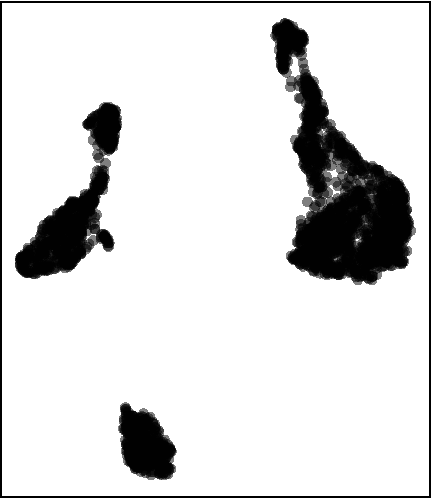
\includegraphics{paper_files/figure-pdf/fig-umapauthor-1.pdf}

}

\caption{\label{fig-umapauthor}2D layout from UMAP (n\_neighbors = 30,
min\_dist = 0.3) applied for the PBMC3k dataset. Is this a best
representation of the original data?}

\end{figure}

\hypertarget{method}{%
\section{Method}\label{method}}

\begin{itemize}
\tightlist
\item
  Create a representation of the model
\item
  Algorithm in 2D

  \begin{itemize}
  \tightlist
  \item
    Parameters
  \item
    Tuning
  \end{itemize}
\item
  Showing model in high-d
\item
  What is learned about simulated examples
\end{itemize}

\hypertarget{applications}{%
\section{Applications}\label{applications}}

\hypertarget{pbmc}{%
\subsection{pbmc}\label{pbmc}}

\begin{verbatim}
 - NLDR view used to illustrate clusters
 - Use our method to assess is it a reasonable representation
 - Demonstrate that it is not
 - Illustrate how to use out method to get a better representation
 
\end{verbatim}

\hypertarget{digits-1}{%
\subsection{digits: 1}\label{digits-1}}

\begin{verbatim}
 - NLDR is used to illustrate different ways 1's are drawn
 - Use our method to assess is it a reasonable representation
 - Demonstrate that it is, except for the anomalies 
 
\end{verbatim}

\hypertarget{discussion}{%
\section{Discussion}\label{discussion}}

\begin{itemize}
\tightlist
\item
  Summarise contributions
\item
  Explain where it is expected or not expected to work, eg higher
  dimensional relationships
\item
  What might be useful enhancements
\end{itemize}

\hypertarget{references}{%
\section*{References}\label{references}}
\addcontentsline{toc}{section}{References}

\renewcommand{\bibsection}{}
\bibliography{bibliography.bib}

\newpage{}




\end{document}
